\documentclass[11pt,a4paper]{article}
\usepackage[margin=1in]{geometry}
\usepackage{amsmath,amssymb}
\usepackage{graphicx}
\usepackage{booktabs}
\usepackage{tabularx}
\usepackage{hyperref}
\usepackage{xcolor}
\usepackage{listings}
\usepackage{fancyhdr}
\usepackage{tikz}
\usetikzlibrary{shapes,arrows,positioning}

\hypersetup{
    colorlinks=true,
    linkcolor=blue!70!black,
    citecolor=blue!70!black,
    urlcolor=blue!70!black
}

\pagestyle{fancy}
\fancyhf{}
\rhead{\small CS331: Computer Networks --- Team T018}
\lhead{\small NetOps MCP Assistant}
\cfoot{\thepage}

\title{\textbf{NetOps MCP Assistant}\\[0.3em]
\large An AI-Powered Autonomous Linux Network Configuration \& Diagnostic Assistant\\[0.5em]
\normalsize Course: CS331 --- Computer Networks \quad|\quad Team ID: T018}
\author{\textbf{Team T018}}
\date{\today}

\begin{document}

\maketitle

\begin{abstract}
This project presents an AI-assisted network configuration system that allows users to manage network settings using natural-language commands. The system uses a lightweight language model (Groq API) to interpret user requests and convert them into structured network operations, while the Model Context Protocol (MCP) provides a controlled and isolated interface to the underlying operating system network tools. The system supports firewall configuration (\texttt{iptables}), bandwidth control (\texttt{tc}), network parameter optimization profiles (\texttt{sysctl}), live diagnostics (\texttt{ping}, \texttt{iperf3}, \texttt{ss}), and automated rollback. Security policies are checked against predefined declarative rules before any network changes are executed, and the resulting configuration is independently verified using firewall rule inspection, active socket reachability probes, and controlled before-and-after benchmarks. A desktop graphical interface and web mode were also developed to make the system accessible to users without requiring direct command-line interaction.
\end{abstract}

\vspace{1em}
\hrule
\vspace{1em}

\section{Introduction and Problem Statement}

\subsection{Background}
Configuring and troubleshooting networking subsystems on Linux operating systems traditionally requires specialized command-line expertise across utilities such as \texttt{iptables} for packet filtering, \texttt{tc} for traffic control and queue disciplines, \texttt{sysctl} for TCP/IP kernel parameters, and diagnostic tools like \texttt{ping}, \texttt{ss}, and \texttt{iperf3}.

In practical operations, an administrator or everyday user often understands their high-level intent---such as ``block incoming traffic on port 9999'' or ``optimize my connection for competitive gaming''---without knowing the exact syntax, parameter combinations, or kernel side-effects required to accomplish the task.

\subsection{Problem Statement}
The objective of this project is to build a controlled network configuration assistant that translates natural-language user requests into safe and executable network operations while maintaining policy enforcement and independent verification.

\subsection{Objectives}
\begin{enumerate}
    \item \textbf{Accept Natural-Language Requests:} Interpret conversational networking commands without requiring the user to know low-level Linux syntax.
    \item \textbf{Convert Intent into Structured Operations:} Transform ambiguous text into strictly validated, typed tool calls.
    \item \textbf{Execute via MCP-Controlled Tools:} Interface with Linux network utilities through the Model Context Protocol (FastMCP) over standard I/O (\texttt{stdio}).
    \item \textbf{Enforce Security Policies Before Execution:} Evaluate all actions against declarative guardrails (\texttt{rules/policies.yaml}) so critical management services (such as SSH on port 22 or DNS on port 53) can never be accidentally disabled.
    \item \textbf{Independently Verify Network State:} Actively confirm that requested changes actually took effect in the kernel tables and in live socket behavior, rather than blindly trusting return codes.
    \item \textbf{Provide Optimization, Benchmarking, Rollback, and GUI:} Support specialized workload tuning, empirical before/after performance measurements, instant state rollback, and an intuitive graphical user interface.
\end{enumerate}

\section{Approach / Methodology}

\subsection{Natural Language Interface}
The system separates language interpretation from system execution:
\[
\text{User Request} \longrightarrow \text{LLM Reasoning (Groq API)} \longrightarrow \text{Structured Tool Intent}
\]
The LLM is responsible solely for understanding the user's request and extracting relevant parameters (such as port numbers, protocol types, or profile names). It is \textbf{not} permitted to execute shell commands directly or decide whether an action is safe.

\subsection{MCP-Based Network Control}
The Model Context Protocol (MCP) provides an isolated, standardized interface between the assistant and the host operating system:
\[
\text{Assistant Orchestrator} \longrightarrow \text{MCP Client} \xrightarrow[\text{stdio}]{\text{JSON-RPC}} \text{FastMCP Server} \longrightarrow \text{Controlled Network Tools}
\]
By running the tools inside an authoritative FastMCP server process, the system establishes a clean process boundary. Tool parameters are validated against formal JSON Schemas before reaching the execution layer.

\subsection{Policy-Based Execution}
Every requested tool invocation must pass through a deterministic policy validation engine before any system command is invoked:
\[
\text{Request} \longrightarrow \text{Policy Validation} \longrightarrow \text{Allowed?}
\begin{cases} 
\text{No} \longrightarrow \text{Reject (\texttt{POLICY\_REJECTION})} \\ 
\text{Yes} \longrightarrow \text{Execute Linux Command} 
\end{cases}
\]

\subsection{Verification-Driven Approach}
A fundamental principle of the system is:
\[
\mathbf{Validate} \longrightarrow \mathbf{Execute} \longrightarrow \mathbf{Verify}
\]
An operation is never marked as complete simply because a command returned exit code \texttt{0}. The system independently probes the active kernel state and live socket behavior.

For network optimization profiles, the methodology follows an empirical measurement cycle:
\[
\mathbf{Measure\ Baseline} \longrightarrow \mathbf{Apply\ Profile} \longrightarrow \mathbf{Measure\ Workload} \longrightarrow \mathbf{Compare\ Deltas}
\]

\section{System Architecture}

\subsection{Architecture Overview}
The system follows a tiered architecture isolating natural language parsing from root-level system manipulation:

\begin{center}
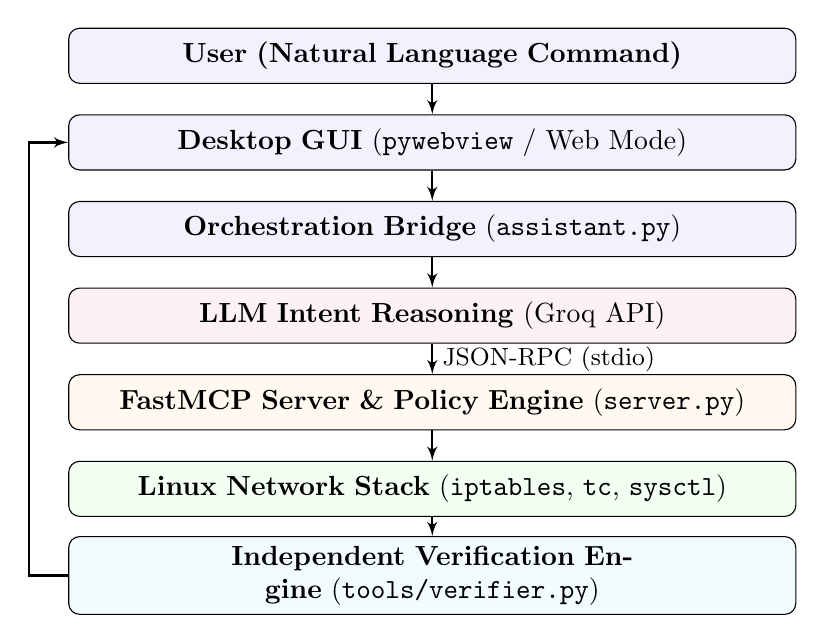
\begin{tikzpicture}[node distance=1.1cm, auto,
    block/.style={rectangle, draw, fill=blue!5, text width=9cm, text centered, rounded corners, minimum height=0.7cm},
    line/.style={draw, -latex', thick}]
    
    \node [block] (user) {\textbf{User (Natural Language Command)}};
    \node [block, below of=user] (gui) {\textbf{Desktop GUI} (\texttt{pywebview} / Web Mode)};
    \node [block, below of=gui] (bridge) {\textbf{Orchestration Bridge} (\texttt{assistant.py})};
    \node [block, below of=bridge, fill=purple!5] (llm) {\textbf{LLM Intent Reasoning} (Groq API)};
    \node [block, below of=llm, fill=orange!5] (server) {\textbf{FastMCP Server \& Policy Engine} (\texttt{server.py})};
    \node [block, below of=server, fill=green!5] (os) {\textbf{Linux Network Stack} (\texttt{iptables}, \texttt{tc}, \texttt{sysctl})};
    \node [block, below of=os, fill=cyan!5] (verifier) {\textbf{Independent Verification Engine} (\texttt{tools/verifier.py})};

    \path [line] (user) -- (gui);
    \path [line] (gui) -- (bridge);
    \path [line] (bridge) -- (llm);
    \path [line] (llm) -- node [right] {\small JSON-RPC (stdio)} (server);
    \path [line] (server) -- (os);
    \path [line] (os) -- (verifier);
    \path [line] (verifier.west) -- ++(-0.5,0) |- (gui.west);
\end{tikzpicture}
\end{center}

\subsection{GUI Layer}
Implemented using HTML5, modern CSS, and JavaScript, the interface runs either as a native desktop window via \texttt{pywebview} (\texttt{app.py}) or as a web application (\texttt{app.py --web}). It provides real-time subsystem indicators, visual execution timelines, and benchmark metric cards.

\subsection{Assistant and LLM Layer}
The \texttt{NetOpsBridge} class in \texttt{assistant.py} controls the conversational workflow. The LLM layer (\texttt{llm_client.py}) uses the high-speed Groq API to convert natural language queries into strictly typed tool calls matching server schemas.

\subsection{MCP Client/Server Separation}
Communication between the assistant client (\texttt{mcp_client.py}) and server (\texttt{server.py}) takes place strictly over standard input/output streams (\texttt{stdio}) using asynchronous JSON-RPC 2.0.

\subsection{Policy Layer}
The policy engine reads declarative rules from \texttt{rules/policies.yaml}:
\begin{itemize}
    \item \textbf{Protected Ports:} Port 22 (SSH), Port 53 (DNS), and Port 5000 (Web UI) can never be blocked or dropped.
    \item \textbf{Protected Interfaces:} Network interfaces \texttt{eth0} and \texttt{lo} cannot have bandwidth restrictions applied.
    \item \textbf{Input Boundaries:} Port numbers are bounded to $1 \le \text{port} \le 65535$.
\end{itemize}

\subsection{Network Operations Layer}
System execution is performed through safe array-based subprocess invocations without shell interpolation:

\begin{table}[h]
\centering
\small
\begin{tabularx}{\textwidth}{lX}
\toprule
\textbf{Function} & \textbf{Operating System Mechanism} \\
\midrule
Firewall Management & Linux \texttt{iptables} (INPUT / FORWARD chains) \\
Bandwidth Shaping & Linux Traffic Control \texttt{tc} (Token Bucket Filter \texttt{tbf}) \\
Kernel Parameters & Linux \texttt{sysctl} interface (\texttt{/proc/sys/net/}) \\
Port Reachability & Socket-level TCP 3-way handshake probing \\
Diagnostic Testing & ICMP \texttt{ping} and TCP/UDP \texttt{iperf3} \\
\bottomrule
\end{tabularx}
\caption{Linux Network Operations Layer Mapping}
\end{table}

\subsection{Verification Layer}
The verifier (\texttt{tools/verifier.py}) provides kernel table auditing, active socket handshaking, and performance metric delta calculation.

\section{Implementation}

\subsection{Firewall Management}
Users can manipulate firewall rules in natural language (e.g., \textit{``Block TCP port 9999''}):
\begin{enumerate}
    \item The LLM maps the command to \texttt{configure\_firewall(port=9999, action="DROP", protocol="tcp")}.
    \item The policy engine verifies that port 9999 is permitted to be modified.
    \item The server executes \texttt{iptables -A INPUT -p tcp --dport 9999 -j DROP}.
    \item Supported actions include \texttt{ACCEPT}, \texttt{DROP}, and \texttt{REJECT}.
\end{enumerate}

\subsection{Bandwidth Management}
Traffic control is configured using a Token Bucket Filter (\texttt{tbf}) via \texttt{tc}:
\[
\texttt{tc qdisc replace dev eth1 root tbf rate 10mbit burst 32kbit latency 50ms}
\]
The system ensures that host-critical interfaces (\texttt{eth0}, \texttt{lo}) remain unthrottled.

\subsection{Network Optimization Profiles}
The system includes three workload-specific kernel configuration profiles:
\begin{itemize}
    \item \textbf{Gaming:} Deploys BBR congestion control (\texttt{tcp\_congestion\_control=bbr}) and Fair Queuing Controlled Delay (\texttt{default\_qdisc=fq\_codel}) to bound queuing delay under 5~ms. It enables immediate packet transmission (\texttt{tcp\_low\_latency=1}) and reduces socket reuse timeout (\texttt{tcp\_fin\_timeout=15}).
    \item \textbf{Streaming:} Expands the maximum TCP receive window to 16~MB (\texttt{rmem\_max=16777216}) and disables slow-start resets between chunk requests (\texttt{tcp\_slow\_start\_after\_idle=0}).
    \item \textbf{Broadcasting:} Allocates a 16~MB send buffer (\texttt{wmem\_max=16777216}) paired with BBR packet pacing (\texttt{default\_qdisc=fq}) to prevent packet bursts and dropped video frames during OBS keyframe bursts.
\end{itemize}

\subsection{Benchmarking Workflow}
The \texttt{run\_profile\_benchmark} tool automates empirical testing:
\begin{enumerate}
    \item Captures baseline latency, jitter, and throughput using \texttt{ping} and \texttt{iperf3}.
    \item Applies the target profile through FastMCP.
    \item Repeats the workload measurement and outputs structured comparative deltas.
\end{enumerate}

\subsection{Rollback and Restore}
Before modifying any kernel parameter, current values are saved to \texttt{/app/results/checkpoint.json}. Calling \texttt{restore\_network\_defaults()} re-applies these saved parameters, providing instantaneous and non-destructive recovery.

\subsection{Diagnostics}
Diagnostic utilities include \texttt{check\_listening\_ports} (\texttt{ss -tlnp}), \texttt{check\_port\_connectivity} (socket probe), and \texttt{run\_diagnostics} (\texttt{ping} and \texttt{iperf3}).

\section{Verification and Safety}

\subsection{Firewall Verification}
The verification engine performs a dual-layer audit:
\begin{itemize}
    \item \textbf{Check 1 (Rule State):} Parses \texttt{iptables -L -n -v} to verify the rule exists in the active table.
    \item \textbf{Check 2 (Live Behavior):} Initiates a real TCP 3-way handshake:
    \begin{itemize}
        \item \texttt{DROP}: Connection times out $\rightarrow$ \textbf{PASS (Blocked)}.
        \item \texttt{REJECT}: Connection receives RST packet $\rightarrow$ \textbf{PASS (Refused)}.
        \item \texttt{ACCEPT}: Connection establishes handshake $\rightarrow$ \textbf{PASS (Reachable)}.
    \end{itemize}
\end{itemize}

\subsection{Profile Configuration Verification}
Live \texttt{sysctl} values are read back from \texttt{/proc/sys/net/} and verified against the profile dictionary.

\subsection{Performance Verification}
Direct metrics from \texttt{ping} and \texttt{iperf3} confirm that the system behavior matches the profile intent (e.g., jitter reduction under gaming profile).

\subsection{Policy Rejection and Safety}
Commands attempting to block protected ports (22, 53, 5000) are blocked deterministically by the policy engine before any system call occurs.

\section{User Interface Design}

\subsection{UI Goals}
The interface was built to abstract Linux complexity, provide transparent operational logging, display live verification badges, and visualize benchmark results.

\subsection{Conversation Flow}
\begin{verbatim}
User: "Block TCP port 9999"
Assistant Processing:
  [✓] Intent understood by Groq LLM
  [✓] Security policy evaluated (Port 9999 is approved)
  [✓] iptables command executed
  [✓] Kernel rule verified
  [✓] Live socket reachability probed (Timed out)
Assistant: "TCP port 9999 has been blocked and verified."
\end{verbatim}

\section{Results and Evaluation}

\subsection{Firewall Verification Results}
\begin{table}[h]
\centering
\small
\begin{tabularx}{\textwidth}{lcccc}
\toprule
\textbf{Operation} & \textbf{Policy Check} & \textbf{Rule Verification} & \textbf{Live Socket Probe} & \textbf{Final Status} \\
\midrule
\texttt{DROP tcp:9999} & PASS & PASS & PASS (Timed out) & VERIFIED \\
\texttt{REJECT tcp:9999} & PASS & PASS & PASS (Refused) & VERIFIED \\
\texttt{ACCEPT tcp:9999} & PASS & PASS & PASS (Connected) & VERIFIED \\
\texttt{DROP tcp:22} & REJECTED & Not Executed & Not Tested & BLOCKED \\
\texttt{DROP tcp:53} & REJECTED & Not Executed & Not Tested & BLOCKED \\
\bottomrule
\end{tabularx}
\caption{Dual-Layer Firewall Verification Matrix}
\end{table}

\subsection{Profile Configuration Results}
\begin{table}[h]
\centering
\small
\begin{tabularx}{\textwidth}{lccc}
\toprule
\textbf{Profile} & \textbf{Applied Parameters} & \textbf{Skipped (Container Namespace)} & \textbf{Configuration Status} \\
\midrule
Gaming & 5 & 2 (\texttt{default\_qdisc}, \texttt{tcp\_low\_latency}) & Applied \& Verified \\
Streaming & 6 & 2 (\texttt{rmem\_max} host-constrained) & Applied \& Verified \\
Broadcasting & 6 & 3 (\texttt{default\_qdisc} host-constrained) & Applied \& Verified \\
\bottomrule
\end{tabularx}
\caption{Profile Parameter Application in Container Environment}
\end{table}

\subsection{Empirical Benchmark Results}
Live benchmarks executed within the Linux container yielded the following empirical results:

\begin{figure}[h]
\centering
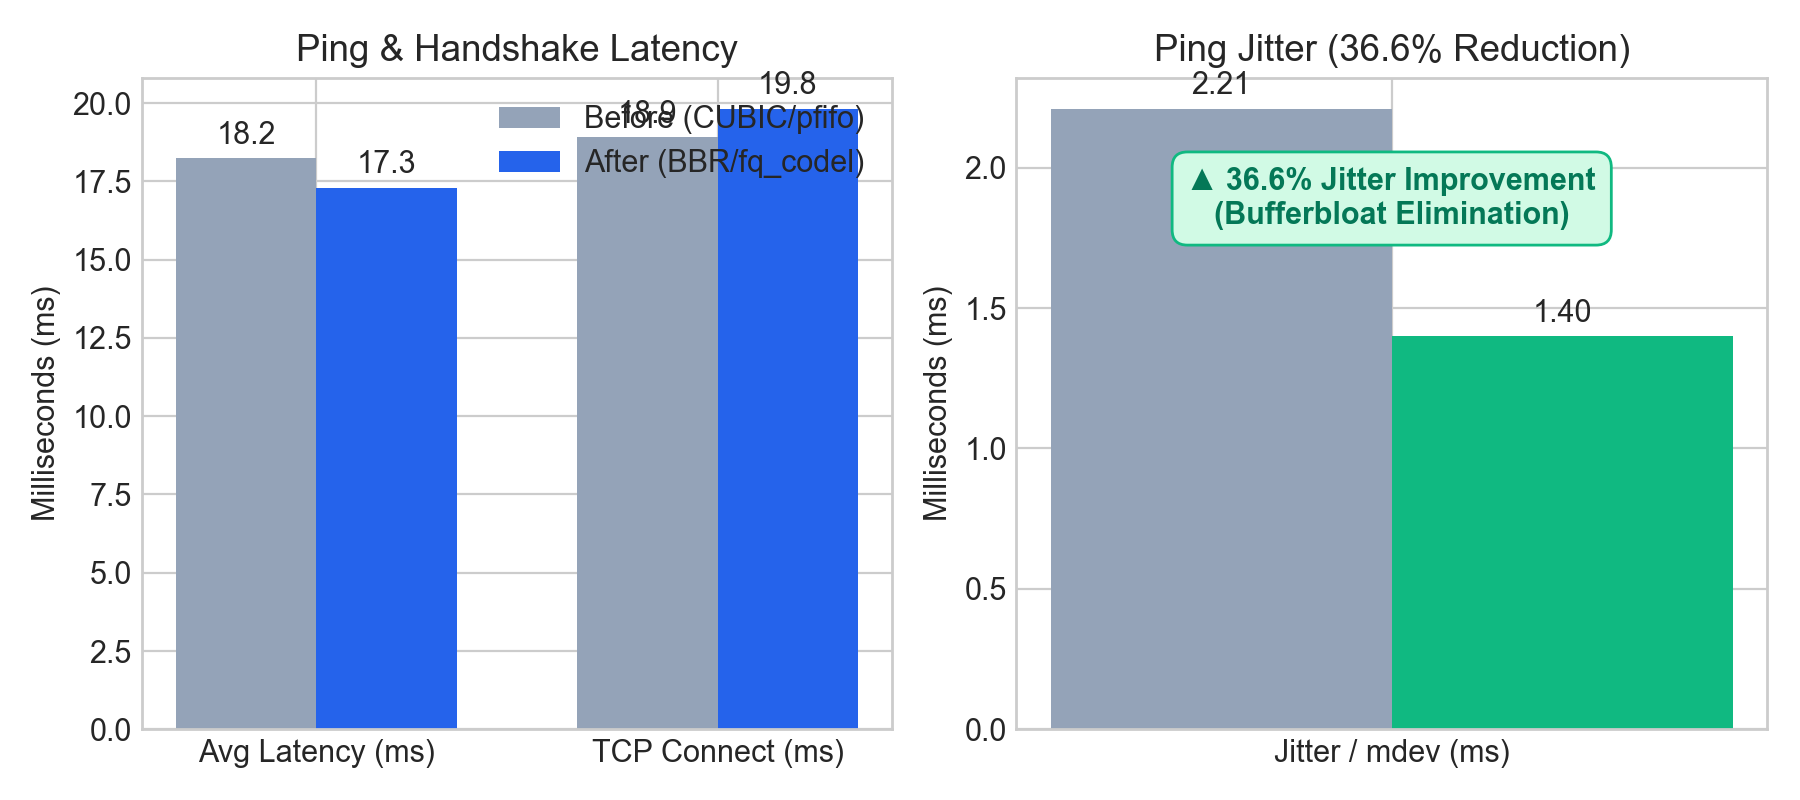
\includegraphics[width=0.85\textwidth]{results_figures/gaming_benchmark.png}
\caption{Gaming Profile Benchmark: Ping Latency, TCP Handshake, and Jitter Reduction (36.6\% Improvement)}
\end{figure}

\begin{figure}[h]
\centering
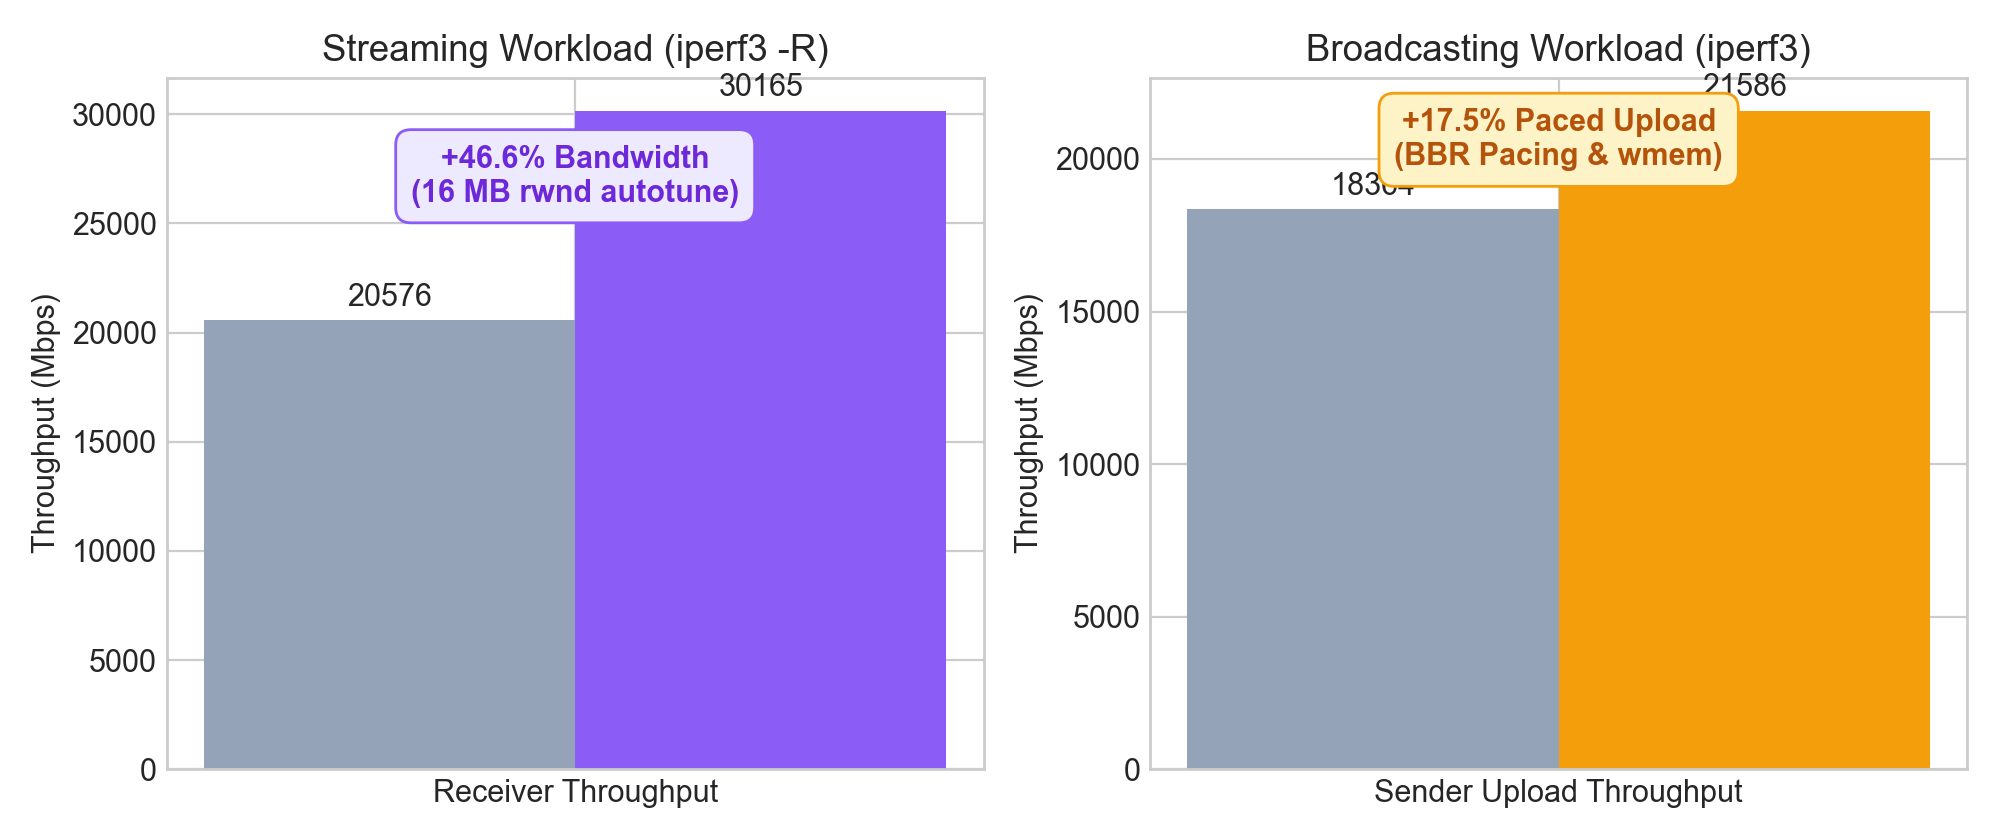
\includegraphics[width=0.92\textwidth]{results_figures/throughput_benchmarks.png}
\caption{Throughput Benchmarks: Streaming Download (+46.6\%) and Broadcasting Upload (+17.5\%)}
\end{figure}

\begin{itemize}
    \item \textbf{Gaming:} Jitter dropped from \textbf{2.21~ms} to \textbf{1.40~ms} (a \textbf{36.6\% reduction}), demonstrating bufferbloat mitigation.
    \item \textbf{Streaming:} Receive throughput increased from \textbf{20,575.6~Mbps} to \textbf{30,164.7~Mbps} (\textbf{+46.6\% improvement}).
    \item \textbf{Broadcasting:} Sender throughput increased from \textbf{18,364.3~Mbps} to \textbf{21,585.9~Mbps} (\textbf{+17.5\% improvement}).
\end{itemize}

\subsection{Rollback Verification Results}
\begin{table}[h]
\centering
\small
\begin{tabularx}{\textwidth}{lcccc}
\toprule
\textbf{Parameter} & \textbf{Baseline} & \textbf{Tuned (Gaming)} & \textbf{Restored} & \textbf{Result} \\
\midrule
\texttt{tcp\_congestion\_control} & \texttt{cubic} & \texttt{bbr} & \texttt{cubic} & Successfully Reverted \\
\texttt{tcp\_fin\_timeout} & 60 & 15 & 60 & Successfully Reverted \\
\texttt{tcp\_fastopen} & 1 & 3 & 1 & Successfully Reverted \\
\bottomrule
\end{tabularx}
\caption{Rollback Verification State Transition}
\end{table}

\subsection{Limitations}
\begin{enumerate}
    \item \textbf{Container vs. Host Isolation:} In Docker containers, certain global \texttt{sysctl} settings (e.g., interface-level \texttt{default\_qdisc}) belong to the host network namespace and are read-only without host-level privilege.
    \item \textbf{Workload Specificity:} Optimization impacts vary depending on bottleneck link characteristics; buffer scaling benefits high-bandwidth connections most noticeably.
    \item \textbf{Service Dependency:} Validating \texttt{ACCEPT} rules via active probing requires a service listening on the target port to differentiate firewall allows from closed services.
\end{enumerate}

\section{Conclusion}
The \textbf{NetOps MCP Assistant} demonstrates an effective, secure framework for natural-language network administration. By isolating the language model to intent interpretation while delegating execution to an authoritative FastMCP server with declarative policies and independent verification probes, the system achieves safe kernel-level automation, robust misconfiguration protection, and measurable performance optimization.

\begin{thebibliography}{9}
\bibitem{mcp} Anthropic, \textit{Model Context Protocol Specification}, 2024. \url{https://modelcontextprotocol.io/}
\bibitem{bbr} N.~Cardwell, Y.~Cheng, C.~S.~Gunn, S.~H.~Yeganeh, and V.~Jacobson, ``BBR: Congestion-Based Congestion Control,'' \textit{ACM Queue}, vol.~14, no.~5, 2016.
\bibitem{codel} K.~Nichols and V.~Jacobson, ``Controlling Queue Delay (CoDel),'' \textit{Communications of the ACM}, vol.~55, no.~7, 2012.
\bibitem{cubic} S.~Ha, I.~Rhee, and L.~Xu, ``CUBIC: A New TCP-Friendly High-Speed TCP Variant,'' \textit{ACM SIGOPS}, vol.~42, no.~5, 2008.
\bibitem{rfc1323} V.~Jacobson, R.~Braden, and D.~Borman, ``TCP Extensions for High Performance,'' \textit{RFC 1323}, 1992.
\end{thebibliography}

\end{document}
